As described in the previous chapter, ECF Modules are the most essential part of the EasyFly programming environment. 
In this chapter, we will analyze each ECF Module available in the EasyFly extension in detail, describing the purpose, main functionalities, and implementation details for each. 
We will first analyze the Modules with an internal state and then move to the Modules with a sensed data state. 

\section{State Estimate Module}\label{sec:module_state_estimate}

Regardless of the purpose, a crucial aspect of operating a drone is having a deep understanding of the drone's position, velocity, and acceleration. 
These parameters are vital for ensuring the drone's stability and safe navigation. 
Accurate knowledge of the drone's position and speed enables its operator to control its movements and avoid obstacles or hazards in its path. 
Furthermore, understanding acceleration is crucial in achieving precision and accurate control of the drone's movements.
State estimate accuracy depends on how much information the control loop can use. 
In particular, the decks that contribute more to the estimation process are the Lighthouse positioning Deck and the Flow Deck V2. 

As the name suggests, the State Estimate Module is an ECF Module that manages the estimated variables of the Crazyflie 2.1.
The full state of the State Estimate ECF Module is:
\begin{lstlisting}[language=Python]
State = {
    "x" : "Position on the x axis from the origin",
    "y" : "Position on the y axis from the origin",
    "z" : "Position on the z axis from the origin",
    "vx" : "Velocity on the x axis",
    "vy" : "Velocity on the y axis",
    "vz" : "Velocity on the z axis",
    "ax" : "Acceleration on the x axis",
    "ay" : "Acceleration on the y axis",
    "az" : "Acceleration on the z axis",
    "roll" : "Roll in rad",
    "pitch" : "Pitch in rad",
    "yaw" : "Yaw in rad",
    "rateRoll" : "Roll rate in rad/s",
    "ratePitch" : "Pitch rate in rad/s",
    "rateYaw" : "Yaw rate in rad/s",
}
\end{lstlisting}

Because the control loop onboard the Crazyflie 2.1 runs at 500Hz, a new estimation is computed every two milliseconds; these variables can rapidly change over time. 
We need to update the state as frequently as possible to ensure that the information provided is accurate and precise. 
For this reason, we selected the lowest possible sampling period for the Communication Framework, which is 10 milliseconds.


In this ECF Module, the utility functions allow the user to record the state variable and, at the end of the flight, plot the recorded data.
As with any other telemetry data, it is usually vital for a user to have the possibility to analyze that information after the flight, especially in the development phase of the application.
For this reason, the utility functions that we implemented will allow a user to analyze and compare data from multiple application runs.


\section{Battery Module Module}\label{sec:module_battery}

When dealing with drones, battery management is an important factor that must always be considered. 
Usually, due to its weight, the battery has minimal capacity, especially on drones with small dimensions.

An application can be perfectly developed, but it can easily fail if it does not consider the limitation of resources like the battery.
To help the developer with this task, we created another ECF Module that manages battery-related information and keeps them updated.

Given this, the full state of the Battery ECF Module is:
\begin{lstlisting}[language=Python]
State = {
	"pm_state" : "Battery power management state",
	"voltage" : "Battery voltage in V",
	"battery_level" : "Estimated battery level in percentage",
}
\end{lstlisting}

The first variable of the state, \textit{pm\_state}, represents the state in which the power management of the drone is in.
The state can be one of the following:
\begin{itemize}
    \item Battery -- The drone is on and using its battery.
    \item Charging -- The drone is plugged into the power supply.
    \item Charged -- The drone has completed the recharge, and its battery is fully charged.
    \item Low Power -- The drone needs to be recharged.
    \item Shutdown -- The drone is off.
\end{itemize}

With the other two properties of the state, \textit{voltage} and \textit{battery\_level}, the developer can determine with high precision the recharging phase.

Since battery management strictly depends on the application to be developed, it is hard to find an implementation that satisfies all the possible usage.
For this reason, we decided to leave the implementation of the decision processes for determining the outside of the Battery Module. 
The module is responsible only for keeping the information in the state consistent and updated.

\section{Multiranger Module}\label{sec:module_multiranger}

The Multiranger deck is an accessory board for the Crazyflie 2.1. 
The deck is designed to provide the drone with range-sensing capabilities, allowing it to detect objects and obstacles in its environment.

The Multiranger deck features four integrated ultrasonic sensors, which can be used to measure distances in a range of up to 5 meters. 
These sensors emit high-frequency sound waves that bounce off of nearby objects and return to the deck, allowing the deck to calculate the distance to the objects based on the time it takes for the sound waves to return.
Multiranger deck is a powerful tool for adding range sensing capabilities to the Crazyflie 2.1, enabling it to perform a range of applications such as mapping, autonomous navigation, and obstacle avoidance.

As any other ECF Module, also the Multiranger Module has a state that it manages. The state is composed of the 5 range measurement, one for each direction that it supports:
\begin{lstlisting}[language=Python]
State: {
    "front" : "Distance from the nearest obstacle on the front (up to 5m)",
    "back" : Distance from the nearest obstacle on the back (up to 5m)",
    "right" : Distance from the nearest obstacle on the right (up to 5m)",
    "left" : Distance from the nearest obstacle on the left (up to 5m)",
    "up" : Distance from the nearest obstacle above (up to 5m)",
}
\end{lstlisting}

Given the wide range of applications the Multiranger deck fits, we decided to implement a simple implementation of two use cases of this deck directly inside the module:
\begin{itemize}
    \item Object Tracking 
    \item Obstacle Avoidance
\end{itemize}


With the Object Tracking behavior, the drone searches for an object to track when it starts. 
As soon it detects an object inside a configurable range, that object becomes the guide to follow. 
The drone with this behavior will try to follow whenever the tracked object moves in space. 

The velocity needs to change depending on the distance from the object. 
If the object is on the perimeter of the activation range, we need to move fast towards it, trying not to lose the tracking. 
On the other hand, when the object is closer to the safe range, the velocity can be slowed since the object is closer to the drone.

When the tracked object stops standing at a fixed point, the drone will get closer to a safe distance that will never be violated.

In summary, as we can see in Figure~\ref{fig:multiranger_tracking}, the drone with an Object Tracking behavior has two ranges:
The first range, which is the activation range, is used to determine what the tracked object is.
The second range, the safety range, is used to prevent collision with the tracked object when it stands at a fixed point.

\sidecaptionvpos{figure}{c}
\begin{SCfigure}[\sidecaptionrelwidth][h]
    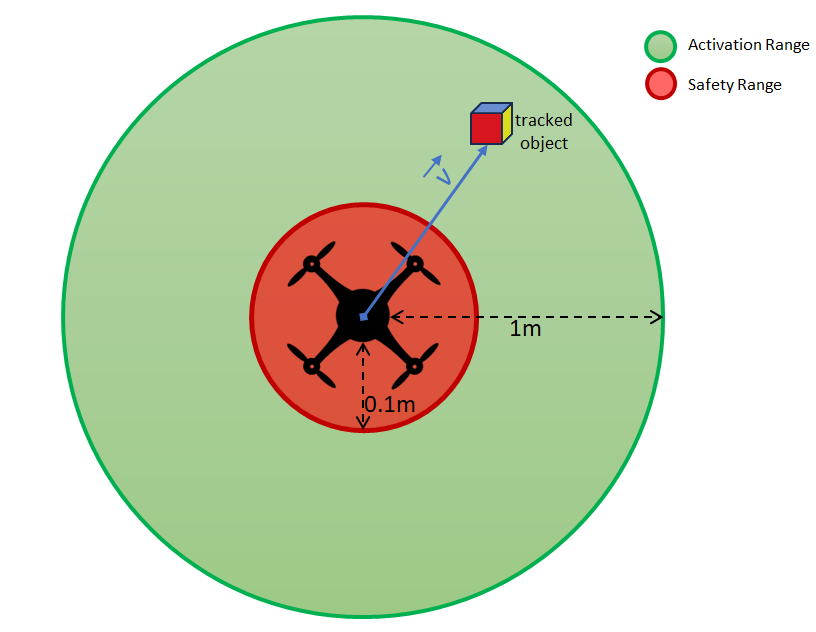
\includegraphics[width=0.5\textwidth]{modules/multiranger}
    \caption{Multiranger Object Tracking behavior}\label{fig:multiranger_tracking}
\end{SCfigure}

The Obstacle Avoidance behavior is the opposite behavior with respect to object tracking. 
In this case, the activation range is used to determine an obstacle to fly away from.

When an obstacle is detected on the perimeter of the activation range, the drone will slowly start moving in the opposite direction. 
If the obstacle is dynamic and gets closer, the drone will increase its speed to try to escape from the obstacle.

In this behavior, the safety limit is used for landing the drone. 
If the obstacle gets too close, the only thing the drone can do to avoid the collision is landing.

\section{Height Module}\label{sec:module_height}

The height module is a 
This deck can measure distances up to 2 meters with an accuracy of around 1 centimeter, making it ideal for altitude sensing tasks in drones applications such as height control, landing, and takeoff.

\section{Lighthouse Module}\label{sec:module_lighthouse}



\section{AI deck Module}\label{sec:module_ai_deck}